\chapter{Grundlagen}

\printmyminitoc{1}

\section{CAN-Bus}
Bei einem CAN-Bus handelt es sich um eine serielle Netzwerktechnologie, 
die mehrere Geräte mit einem Draht verbindet.
Die Entwicklung des CAN-Bus wurde von Bosch im Jahr 1983 begonnen. Im Jahr 1986 wurde der erste CAN-Bus Standard 
veröffentlicht.
Die Motivation der Entwicklung war die effiziente Kommunikation zwischen den Steuergeräten in einem Auto. 
Als günstige
Nebenwirkung konnte damit die Kabelmenge reduziert werden, da alle Geräte mit einem Bus verbunden werden können.
Durch die höhere Zuverlässigkeit und Funktionalität des Can-Bus, wurde dieser schnell in der Autoindustrie etabliert.
Aber auch in anderen Sektoren, wie z.B. der Medizintechnik, der Gebäudeautomation oder der Luftfahrt, spielt der
Can-Bus mittlwerweile eine wichtige Rolle.
\cite[Seiten 2-10]{Voss2008}
\\
Man sprich von einem Bussystem, da mehrere Geräte miteinander über diesen miteinander verbunden werden. 
Die Geräte auf an dem Bus sind in dem Fall die Knoten. Alle sind gleichberechtigt und können Nachrichten senden und empfangen.
Die Nachrichten werden nach Broadcasting-Prinzip übertragen. Dabei wird jede Nachricht von allen Knoten empfangen, 
aber nur die Knoten, welche die Nachricht benötigen, verarbeiten sie. 
Die Nachrichten werden nicht auf Einhaltung der Protokollregeln 
überprüft, da dies zu einer größeren unnötigen Last auf dem Bus führen würde. 
Jedoch wird die Integrität der Nachrichten durch eine Prüfsumme sichergestellt. Das wird auch mit 
einer Acknowledge-Nachricht(ACK) bestätigt. Wird eine Nachricht nicht bestätigt, wird von dem Sender eine Fehlermeldung
auf den Bus gesendet.
Bei einer fehlerhaften Nachricht sendet der Empfänger eine Fehlermeldung, die wieder von allen Knoten empfangen wird.
Wenn ein Knoten dauerhaft fehlerhafte
Nachrichten sendet, wird er vom Bus getrennt. Die auf den Bus gesendeten Daten werden mit einer Nachrichten-ID
versehen, welche die Priorität der Nachricht angibt. Die Nachrichten mit der niedrigsten ID haben die höchste Priorität.
Die Maximale Länge einer Nachricht beträgt 8 Byte. 
Auf dem CAN-Bus kann eine maximale Baudrate von 1Mbit/s erreicht werden.
Zusätzlich kann durch die geringe Länge der Nachrichten geringe Latenz erreicht werden. 
Insgesamt ist der CAN-Bus damit gut für Echtzeitanwendungen geeignet, da die Reaktionszeit der Knoten möglichst gering gehalten wird.
\cite[Seiten 13-19]{Voss2008}
\\
Alle Knoten in einem Can-Bus sind mit einem zweiadrigen Kabel verbunden. Diese werden als High(CAN\_H) und Low(CAN\_L) 
bezeichnet. Der Bus ist an beiden Enden mit einem Widerstand von 120 $\Omega$ abgeschlossen, um Reflexionen zu vermeiden.
\cite[Seite 132]{Voss2008}
\\
Eine Nachricht auf einem CAN-Bus ist im allgemeinen in einem Can-Frame verpackt. Dieser beginnt
mit einem Startbit, welches Start of Frame (SOF) genannt wird. Darauf folgt das Arbitration Field, 
in dem die Nachrichten-ID und ein Bit RTR (Remote Transmission Request) gesetzt wird. Das RTR-Bit wird gesetzt,
wenn der Sender eine Antwort auf die Nachricht erwartet. Das Control Field wird für die Datengröße und die Nachrichtenlänge
verwendet. Im Data Field sind die eigentlichen Nutzdaten kodiert. Das CRC Field enthält eine Prüfsumme, welches die Richtigkeit
der Nachricht überprüft. Hier folgt ein ACK Field, welches die Prüfsumme bestätigt. Die Nachricht endet mit einem End of Frame (EOF).
Danacht folgt ein Interframe Space (IFS) von 3 Bit, welches eine Pause zwischen den Nachrichten darstellt.
\cite[Seite 36]{Voss2008}

\subsection{Erweitertes Can-Protokoll}
Das Standard Can-Protokoll hat einen 11 Bit Identifier, während das erweiterte Can-Protokoll 29 Bit Identifier
besitzt.
Die Society of Automotive Engineers (SAE) hat das J1939-Protokoll entwickelt, um die Kommunikation in Nutzfahrzeugen
zu verbessern. Der Fokus liegt auf der Kommunikation mit dem Antrieb des Fahrzeugs. Der 11-Bit-Identifier wird in J1939 
auf 29 Bit erweitert, um eine größere Anzahl verschiedener Nachrichten zu ermöglichen.\\
Auf einem Can-Bus können der Standard 11 Bit Identifier und der erweiterte 29 Bit Identifier gleichzeitig verwendet werden.
Eine Nachricht mit dem 11 Bit Identifier wird bevorzugt vor einer Nachricht mit 29 Bit Identifier, wenn diese die gleiche
Priorität haben. Die spezifierten Baudraten sind hier 250kbit/s und 500kbit/s. Die Hauptkomponenten des
erweiterten Identifier sind die Priority, eine Parameter Group Number (PGN) und eine Quell-Adresse.
Das PGN-Feld ist aus 1 Bit Data Page (DP), 1 Bit Extended Data Page (DP), einer Protocol Data Unit (PDU) und einem PDU spezifischen 
Feld (PS) aufgebaut. Die DP und EDP bestimmen mit welchem Standard die 
Nachricht gesendet wird. Für SAE J1939 werden aber nur zwei Kombinationen verwendet. 
Das PS-Feld kann entweder eine Zieladresse oder eine Gruppenerweiterung (GE) sein. Welches PS-Feld
verwendet wird, hängt von der PDU ab. Wenn diese einen Wert von unter 240 hat, wird das PS-Feld als Zieladresse verwendet. 
In dem anderen Fall wird das PS-Feld als Gruppenerweiterung verwendet.
\cite{Murvay2018}
\begin{figure}[H]
    \centering
    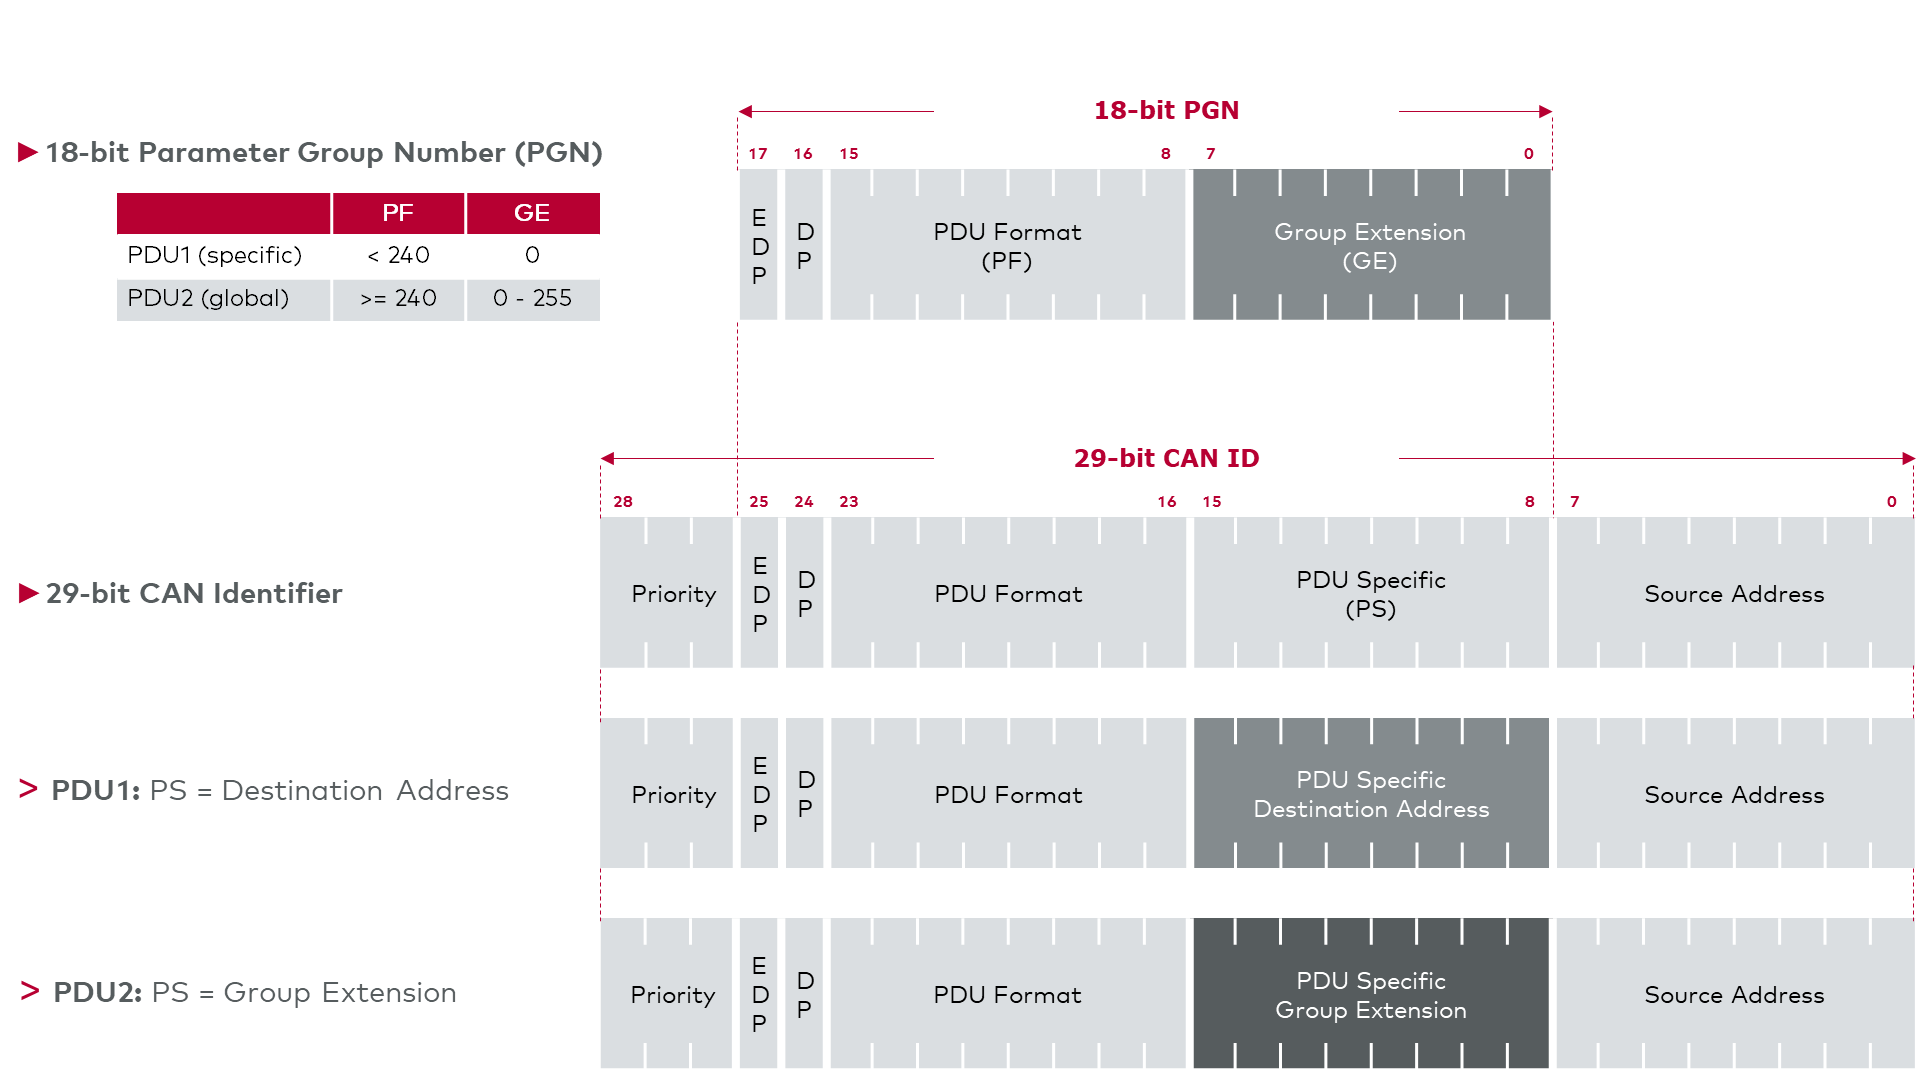
\includegraphics[scale=0.28]{images/j1939header.png}
    \caption{Header einer J1939-Nachricht auf dem CAN-Bus \cite{VectorSAE}(letzter Zugriff: 28.01.2025)}
    \label{fig:j1939header}
\end{figure}

Trotz des Broadcasting-Prinzips soll nicht jede Nachricht von jedem Knoten verarbeitet werden.
Die Zieladresse ermöglicht es, dass eine Nachricht nur von dem designierten Knoten verarbeitet wird.
Um eine Nachricht an alle Knoten 
zu senden, wird die Zieladresse auf 255 gesetzt. Mit der Gruppenerweiterung ist es nicht möglich eine Nachricht 
zielgerichtet an bestimmte Geräte zu senden. \cite{Murvay2018}




\section{Raspberry Pi}
Ein Raspberry Pi ist ein Einplatinencomputer, der von der Raspberry Pi Foundation entwickelt wurde. 
Dieser hat den Prozessor mit Grafikeinheit, Arbeitsspeicher, Speicher und Anschlüssen auf einem einzigen Board integriert.
Es handelt sich um einen vollwertiger Computer, der kleiner als normale PCs ist. Für die Größe ist der Raspberry Pi
leistungsstark. Zusätzlich kann dieser mit einem normalen Betriebssystem
betrieben werden. Das macht ihn zu einem vielseitigen Werkzeug und attraktiv für diese Arbeit.
Trotzdem gibt es ein spezielles Betriebssystem, das für den Raspberry Pi entwickelt wurde, das Raspberry Pi OS (ehemals Raspbian).
Dieses basiert auf der Linux-Distribution Debian. Um viele Funktionen erfüllen zu können, hat der Raspberry Pi viele Anschlüsse.
Der Raspberry Pi 5 hat 4 USB-Anschlüsse, 2 Micro-HDMI-Anschlüsse, 1 Ethernet-Anschluss, 1 USB-C-Anschluss für die Stromversorgung und einen Micro-SD-Kartensteckplatz.

\subsection{Raspberry Pi als Rogue Device}
Unter einem Rogue Device versteht man ein Gerät, das sich unautorisiert und unauffällig in ein Netzwerk integriert. \cite{Scarfone2008}
Dies kann ein Raspberry Pi sein, der sich in ein Netzwerk einbindet und Daten abfängt oder manipuliert. Hierüber können 
sich Angreifer Zugriff auf das Netzwerk verschaffen. 
Ein solches Gerät kann dazu verwendet werden, um eigenen Code auszuführen. Der kann beispielsweise Daten veränden oder 
weitere Angriffe vorbereiten. Zudem kann es von Angreifern aus der Ferne gesteuert werden, wodurch gezielte 
Manipulationen oder Spionageangriffe vereinfacht werden. Darüber hinaus lässt sich ein Rogue Device nutzen, um Informationen 
über das Netzwerk zu sammeln, etwa durch das Mithören von Kommunikation oder die Analyse von Sicherheitsmechanismen.
Das ermöglicht es, Schwachstellen im Netzwerk aufzudecken und gezielt auszunutzen.

\section{State of the Art}
Die Technologie des CAN-Bus ist seit einiger Zeit etabliert und wird in vielen Bereichen eingesetzt.
Daher gibt es auch viele Tools und Bibliotheken, die es ermöglichen, mit dem CAN-Bus zu arbeiten.
In diesem Abschnitt wird der aktuelle Stand der Technik vorgestellt.

\subsection{Anbindung von Raspberry Pi an CanBus}
In der folgenden Arbeit soll ein Raspberry Pi an einen CAN-Bus angeschlossen werden. 
Im Folgenden werden einige verschiede Möglichkeiten vorgestellt.\\
Die erste Möglichkeit ist die Verwendung eines Microchip MCP251x, der als CAN-Controller dient. Dieser wird 
mit dem Microchip MCP2551 ergänzt, der als CAN-Transceiver dient. Diese Kombination ermöglicht es, den
Raspberry Pi mit dem CAN-Bus zu verbinden. Der MCP251x wird über die SPI-Schnittstelle (Serial Peripheral Interface) 
des Raspberry Pi angeschlossen. Dazu wird ein Treiber benötigt, der die Kommunikation zwischen dem Raspberry Pi und dem
MCP251x ermöglicht. Ein solcher Treiber ist bereits seit dem 05.05.2015 im Raspberry Pi OS (ehemals Raspbian OS)
integriert. \cite{Salunkhe2016}
Um diese Möglichkeit zu vereinfachen, gibt es auch verschiedene HATs (Hardware Attached on Top), die solche Microchips
bereits integriert haben. Ein Beispiel dafür ist das PiCan2 von SK Pang Electronics. Dieses Board wird auf den 
GPIO-Pins (General Purpose Input/Output) des Raspberry Pi gesteckt. Es erlaubt dem Raspberry Pi mit dem CAN-Bus
zu kommunizieren. Das PiCan2 unterstützt eine Geschwindigkeit von bis zu 1Mbit/s. \cite{Pant2019}\\
Es besteht auch die Möglichkeit, einen USB-CAN-Adapter zu verwenden. Damit ist die Anbindung eines 
beliebigen Computer an den CAN-Bus möglich.
Ein Beispiel für einen solchen Adapter ist der UCAN von Fysetc. Die Hardware und Firmware des Adapters
sind open-source. Die Verbindung zum Raspberry Pi erfolgt über USB-C.
Zum CAN-Bus müssen lediglich CAN\_H und CAN\_L und die Masse verbunden werden. Mit dem richtigen Treiber funktioniert
dieser Adapter mit Linux, Windows und MacOS.  
\cite{FysetcUCAN} (letzter Zugriff: 17.02.2025)


\subsection{Überseztung von CAN-Nachrichten}
Viele Software Tools ermöglichen die Arbeit mit dem CAN-Bus. Um einen Überblick zu bekommen, 
werden hier einige vorgestellt. Diese Tools unterscheiden sich in ihrem Funktionsumfang, ihrer Benutzerfreundlichkeit 
und den unterstützten Anwendungsfällen. Einige Programme sind speziell für die Analyse und das Debugging von CAN-Nachrichten 
ausgelegt, während andere umfassende Entwicklungs- und Simulationsmöglichkeiten bieten. Im Folgenden werden die wichtigsten 
Eigenschaften, Einsatzbereiche und Besonderheiten der einzelnen Tools vorgestellt. \\
\begin{itemize}
    \item \textbf{canCommander}: Dieses Tool ermöglicht das Senden und Empfangen von CAN-Nachrichten. Es bietet eine einfache 
    Benutzeroberfläche und umfangreiche Analysefunktionen. Mit canCommander können CAN-Nachrichten aufgezeichnet, 
    analysiert und bearbeitet werden. Dabei können auch Nachrichten gesendet und injiziert werden. Es wird auch eine
    schon vorbereitete Platine verkauft, die es ermöglicht, mit dem CAN-Bus zu arbeiten. Dennoch ist canCommander ein
    open-source Projekt und kann auch auf anderen Plattformen verwendet werden. Diese Plattformen beschränken sich aber
    auf Mikrocontroller, wie Arduino Uno oder ESP32. \cite{can_commander} (letzter Zugriff: 15.02.2025)
    \item \textbf{cantools}: Diese Python-Bibliothek ermöglicht es, CAN-Nachrichten zu dekodieren. Mit cantools können 
    CAN-Daten in ein Menschenlesbares Format umgewandelt werden. Die Bibliothek 
    bietet eine Vielzahl von Funktionen und unterstützt verschiedene Protokolle und Datenformate. Damit ist cantools ist ein 
    nützliches Werkzeug für die Analyse und Verarbeitung von CAN-Nachrichten und eignet sich für die Entwicklung von 
    Anwendungen, die mit dem CAN-Bus arbeiten. \cite{cantools} (letzter Zugriff: 15.02.2025)
    \item \textbf{CANoe}: Dieses eigenständige kommerzielle Tool wurde von der Firma Vector Informatik GmbH. entwickelt.
    Es bietet eine vielzahl an verschiedenen Funktionen. CANoe ermöglicht die Entwicklung, Simulation und Analyse von
    CAN-Netzwerken. Es bietet eine umfangreiche Funktionalität und unterstützt verschiedene Protokolle und Datenformate.
    \cite{VectorCANoe} (letzter Zugriff: 15.02.2025)
    \item \textbf{can\_decoder}: Das Open-Source-Projekt ermöglicht das Dekodieren von CAN-Nachrichten. Es wurde von der Firma
    CSS-Electronics entwickelt und ist auf GitHub verfügbar. Allerdings ist das Projekt nicht mehr aktiv und wird nicht mehr
    weiterentwickelt. Trotzdem kann es ein nützliches Werkzeug für die Analyse und Verarbeitung von CAN-Nachrichten sein. 
    \cite{can_decoder} (letzter Zugriff: 15.02.2025)
    \item \textbf{SavvyCAN}: Die C++ Anwendung kann CAN-Nachrichten aufzeichnen, welche durch Reverse-Engineering analysiert werden können.
    Hiermit können auch einzelne Nachrichten dekodiert werden. SavvyCAN ist ein Open-Source-Projekt und kann auf GitHub gefunden werden. Zusätzlich
    gibt es Unterstützung auf Linux und Windows. \cite{SavvyCAN} (letzter Zugriff: 15.02.2025)
    \item \textbf{can-utils}: Diese Set an Linux-Tools ermöglichen die Arbeit mit dem CAN-Bus. Damit ist es möglich, CAN-Nachrichten zu senden und zu empfangen.
    Es ist ein Open-Source-Projekt und kann auf GitHub gefunden werden. Diese Tools bieten eine Grundlage für die Entwicklung von Anwendungen, die mit dem CAN-Bus arbeiten.
    \cite{can-utils} (letzter Zugriff: 15.02.2025)
\end{itemize}
Um der Nutzlast der CAN-Bus Nachrichten Informationen zuzuordnen, ist eine DBC-Datei essentiell. 
Diese Datei schlüsselt auf, welche Informationen in den verschiedenen CAN-Nachrichten enthalten sind.
Da auch sensible Informationen in den Nachrichten enthalten sein können, wird diese Datei in den meisten 
Fällen nicht öffentlich verfügbar gemacht. Ohne diese Datei können zwar Brute-Force Ansätze verwendet werden,
allerdings ist dies sehr aufwendig und nicht zielführend. \cite{Choi2021} \\
Um die vorher genannten Tools zu verwenden, ist es also notwendig, die DBC-Datei zu haben. Bei canCommander
sind einige DBC-Dateien bereits vorinstalliert. Bei cantools kann die DBC-Datei in das Programm geladen werden.
Allerdings kann es eine Schwierigkeit darstellen, die bestimmte DBC-Datei zu erhalten.